\section{Fundamentos Teóricos}

\begin{frame}{Dados de reconstrução}
    
    \textbf{Pointcloud} \only<1>{conjunto de pontos que pertencem à superfície do objeto.}
        \only<1>{
            \begin{itemize}
                \item A mais fácil de obter.
                \item Colorização é feita ponto a ponto.
                \item Não armazena informação semântica sobre o objeto.
                \item Mais resolução implica um crescimento cúbico do numero de pontos.
                \item Propriedades iguais são repetidas por todos os pontos.
            \end{itemize}
        }

    \textbf{Mesh} \only<2>{conjunto de triângulos que formam a superfície do objeto.}

        \only<2>{
            \begin{itemize}
                \item Muito usada em CG.
                \item Colorização é feita por texturas.
                \item Armazena informação semântica, como a área, volume.
                \item Mais realista (occlusão, lightning (reflexões)).
                \item Possibilidade de ser usado em muitos algoritmos (CFD).
                \item Mais resolução não implica um aumento do número de triângulos.
            \end{itemize}
        }


    \textbf{Modelos Semânticos} \only<3>{superfície é modelada por modelos matemáticos.}

    \only<3>{
        \begin{itemize}
            \item Usado em reconstruções de modelos para modelação, fabrico ou para obtenção de modelos simplificados.
            \item Usualmente usadas curvas de Bezier como modelo.
            \item Difícil de automatizar. Requer assim muito processamento manual.
            \item Pouco usado em relação à Mesh.
        \end{itemize}
    }

\end{frame}

\subsubsection{Tecnologias}

\begin{frame}{Visão Estéreo}
				
	\begin{minipage}{0.5\textwidth}
		\begin{itemize}
			\item Mecanismo similar ao funcionamento estéreo do olho humano.
			\item Distância é calculada pelo cálculo da disparidade entre duas imagens. Esta disparidade é depois transformada numa nuvem de pontos.
			\item Não contem informação dimensional absoluta, apenas relativa.
		\end{itemize}
	\end{minipage}%
	\begin{minipage}{0.5\textwidth}
		\begin{figure}
			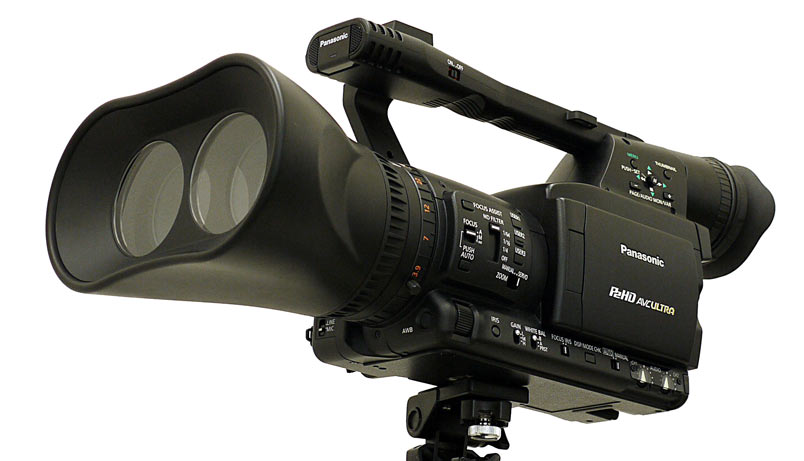
\includegraphics[width=1\textwidth]{img/3d-camera.jpg}
		\end{figure}
	\end{minipage}
						
\end{frame}

\begin{frame}{RGBD}
			
	\begin{minipage}{0.5\textwidth}
		\begin{itemize}
			\item Utiliza um sensor destinado à captura da informação de depth. Usualmente é usado uma câmara IR que capta padrões desenhados por um laser.
			\item Resulta numa imagem com informação de cor (RGB) e distância (D).
			\item Esta tecnologia não é muito precisa.
		\end{itemize}
	\end{minipage}%
	\begin{minipage}{0.5\textwidth}
		\begin{figure}
			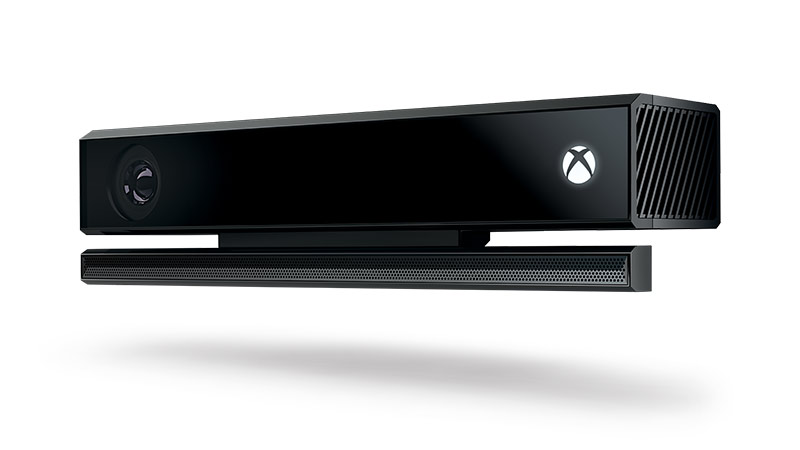
\includegraphics[width=.9\textwidth]{img/kinect.jpg}
		\end{figure}
	\end{minipage}
						
\end{frame}

\begin{frame}{Lidar: Light Detection and Ranging}
						
	\begin{minipage}{0.5\textwidth}
		\begin{itemize}
			\item Usa um sinal laser pulsado para medir distancias.
			\item Muito utilizado para medir a topografia da Terra.
			\item Consegue medições muito precisas ($<1mm$).
			\item Não contêm informação de cor.
		\end{itemize}
	\end{minipage}%
	\begin{minipage}{0.5\textwidth}
		\begin{figure}
			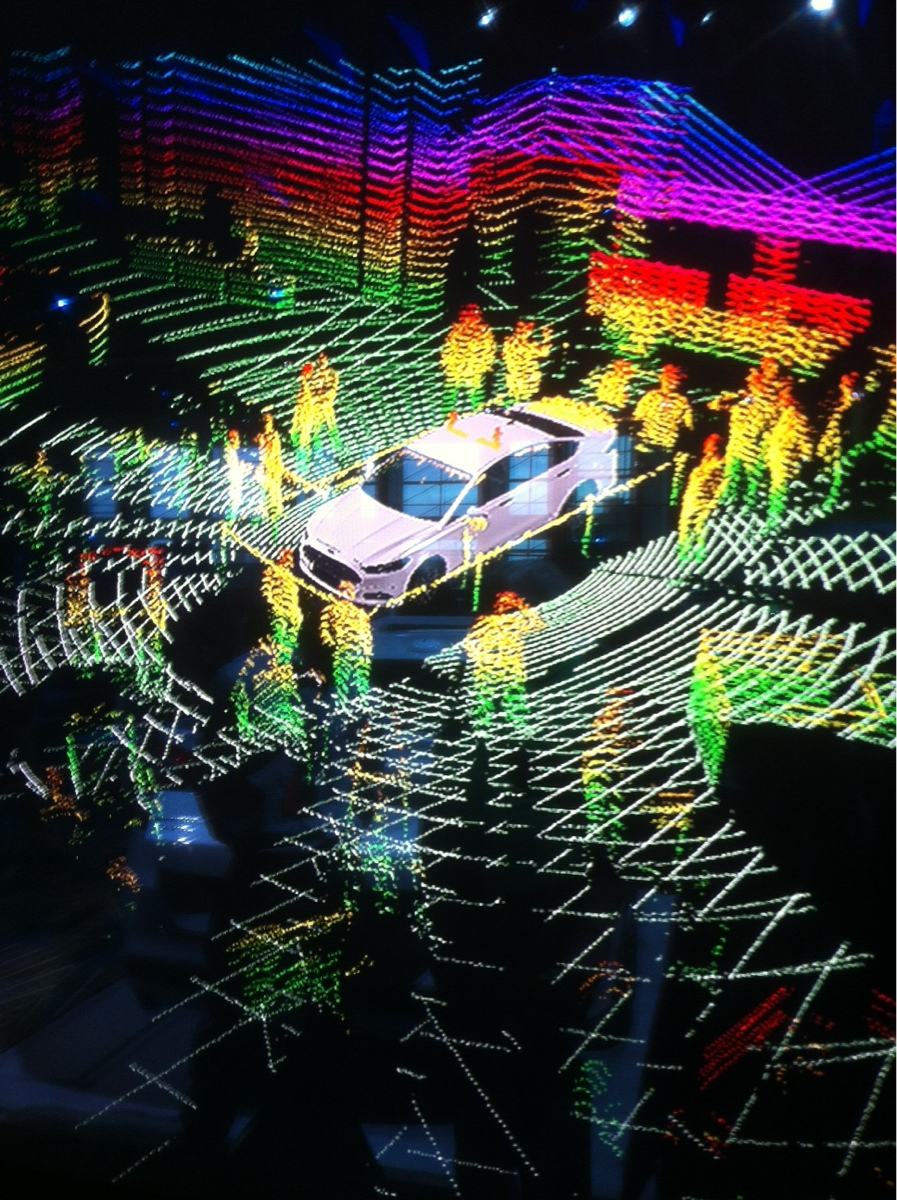
\includegraphics[width=.9\textwidth]{img/lidar.jpg}
		\end{figure}
	\end{minipage}

\end{frame}